\documentclass[a4paper,12pt,openany]{article}
%\documentclass[a4paper,12pt,openany]{book}

\usepackage{hyperref}    
\usepackage{amsmath,amssymb,amsfonts,amsthm,mathtools}    % Typical maths resource packages
\usepackage{alphalph}
\usepackage{graphicx}                           % Packages to allow inclusion of graphics
                       % For creating hyperlinks in cross references
%\usepackage[authoryear]{natbib}                 % literature reference style
\usepackage[font=scriptsize,it,bf, format=hang]{caption}
\usepackage{subcaption}
\usepackage{setspace}
\usepackage{multicol}
\usepackage{upgreek}
\usepackage{multirow} 
\usepackage{float}
\usepackage{changepage}
\usepackage[ngerman]{babel}
\usepackage[utf8]{inputenc}
\usepackage{graphicx}
\usepackage{rotating}
\usepackage{fancybox}
\usepackage{enumerate}
\usepackage[framemethod=TikZ]{mdframed}
\usepackage{xcolor}
\usepackage{etoolbox}
 \usepackage{nccmath}
 \usepackage{adjustbox}
 \usepackage{arydshln}
 \usepackage{moresize}
 \usepackage{booktabs}
 \usepackage{ngerman}
 \usepackage{pdflscape}

\usepackage{mathptmx}
\usepackage{amsthm}
\usepackage{listings}
\usepackage{bm}

\usepackage[a4paper,margin=1cm, lmargin=5cm]{geometry}
\usepackage{tikz} 
 \usepackage{pgflibraryshapes} 
\usetikzlibrary{arrows} 
\usetikzlibrary{positioning} 
\usetikzlibrary{shapes} 
\usetikzlibrary{fit} 
\usetikzlibrary{backgrounds} 
\usepackage{booktabs}
\usetikzlibrary{calc}

\usepackage{pdflscape}

% -------------------------------
% --- some layout definitions ---
% -------------------------------

% define citation style
\usepackage[notocbib]{apacite}
\bibliographystyle{apacite}

% define page size, margin size
\setlength{\headheight}{1\baselineskip}
\setlength{\parindent}{0in}
\voffset=-2cm
\hoffset=-3cm
\textheight24cm
\textwidth15.5cm
\topmargin1cm
\oddsidemargin3cm
\evensidemargin3cm

% define caption spacing
\captionsetup[table]{skip=0pt, font=scriptsize}
\captionsetup[figure]{skip=0pt, font=scriptsize}

% define line line spacing = 1
\renewcommand{\baselinestretch}{1.02}\normalsize

% define second level for `itemizing'
\renewcommand{\labelitemii}{-}

%% new math commands 
\newcommand\independent{\protect\mathpalette{\protect\independenT}{\perp}}
\def\independenT#1#2{\mathrel{\rlap{$#1#2$}\mkern2mu{#1#2}}}

\definecolor{lightgray}{gray}{0.8}
\newcommand{\suchthat}{\;\ifnum\currentgrouptype=16 \middle\fi|\;}

% define Theorem, Definition and Example labeling
%\theoremstyle{plain}
%\newtheorem{thm}{Theorem} % reset theorem numbering for each chapter
%\theoremstyle{definition}
%\newtheorem{defn}{Definition}[chapter]

%%%%%%%%%%%%%%%%%%%% Main document --------------------------------------

\begin{document}

\pagestyle{plain}
\setcounter{page}{1}  
\pagenumbering{arabic}  


%%%%%%%%%%%%% Inputs

\section{Single construct models}

\subsection{Models and coefficients}

Two parallel test halves were build, corresponding to sum scores of half of the trials of the same time point per task. Trials were alternately assigned to the first and the second test half. For tasks repeated 12 times per measurement time point this procedure resulted in two test halves assuming 7 possible values (0 to 6 correctly solved trials), for tasks repeated 8 times per measurement time point test halves could maximally assume 5 possible values (0 to 4 correctly solved trials). Not all categories were observed at all time points and categories had to be collapsed in some cases (see descriptions below). The two test halves served as indicators for a common latent construct per measurement time point, assuming parallel test halves (i.e., factor loadings set to 1 and assuming equal reliabilities). Due to only few observed categories, indicators were modeled as ordered categorical, using a probit link function. The models thereby correspond to Graded response models. For model parsimony, to improve estimation accuracy (see simulation studies) and in order to test for latent mean differences across time, thresholds for all indicators were set equal across time (resulting in the assumption of strict measurement invariance) as well as across test halves.

\subsubsection{Latent State models}

\textbf{Measurement Equation}

Measurement equation for parcel $i$ at time point $t$:
\begin{equation}
Y_{it}= S_t + \epsilon_{it}
\end{equation}

At each time point $t$, a latent state variable $S_t$, underlying the two observed indicators $Y_{1t}$ and $Y_{it}$ is estimated. Latent state variables are allowed to freely correlate across time, with latent (measurement-error free) correlations serving as indirect indicators of stability across time. The model is depicted for 6 measurement time points in Figure \ref{Fig: LS graph}. 

%%%% Insert model graphic LS model
\begin{figure}[!h]
\begin{center}
\resizebox{0.35\columnwidth}{!}{%
\begin{tikzpicture}
        [manifest/.style={rectangle,draw=black!80,semithick,minimum width=1.5cm,inner sep=
4pt,text centered},
        latent/.style={ellipse,draw=black!80,thick,inner sep=2,text centered},
        on/.style={->,>=stealth',semithick},
        from/.style={<-,>=stealth',semithick},
        with1/.style={<->,>=stealth',semithick,bend left=30},
        with2/.style={<->,>=stealth',semithick,bend right=30},
        with3/.style={<->,>=stealth',semithick,bend left=50},]

% Latent Variables %
 \begin{scope}[node distance=1.5]
                \node[latent] (o1) at (0,0) {$S_{1}$};
                \node[latent] (o2) [below=of o1] {$S_{2}$};
                \node[latent] (o3) [below=of o2] {$S_{3}$};
                \node[latent] (o4) [below=of o3] {$S_{4}$};
                \node[latent] (o5) [below=of o4] {$S_{5}$};
                \node[latent] (o6) [below=of o5] {$S_{6}$};
\end{scope}
                                                             	                        
% Manifest % 
 \foreach \a in {1,...,6} {\node (y1\a) [right = 2 of o\a] (yhelp\a) {};}        
 \foreach \b in {1,...,6} {\node[manifest] [above = .05 of yhelp\b] (y1\b) {$Y_{1\b}$}
 	edge [from] node[above] {1} (o\b);}
 \foreach \c in {1,...,6} {\node[manifest] [below = .05 of yhelp\c] (y2\c) {$Y_{2\c}$}
 	edge [from] node[below] {$1$} (o\c);} 

% Fehler %
\foreach \a in {1,...,5} {\node (e1\a) [below right = .3 of y1\a] {}
	edge [on] (y1\a.south east);}
\foreach \b in {1,...,5} {\node (e2\b) [below right = .3 of y2\b] {}
	edge [on] (y2\b.south east);}

\node (e16) [below right = .3 of y16] {$\epsilon_{16}$}
	edge [on] (y16.south east);
\node (e26) [below right = .3 of y26] {$\epsilon_{26}$}
	edge [on] (y26.south east);

%correlations%
\foreach \a in {1,...,5} {
\draw[<->,>=stealth',semithick] (o\a) to [with2]
node[align=center,below,yshift= 0mm, pos=0.5] 
                      {}  (o6);}
\foreach \a in {1,...,4} {
\draw[<->,>=stealth',semithick] (o\a) to [with2]
node[align=center,below,yshift= 0mm, pos=0.5] 
                      {}  (o5);}
\foreach \a in {1,...,3} {
\draw[<->,>=stealth',semithick] (o\a) to [with2]
node[align=center,below,yshift= 0mm, pos=0.5] 
                      {}  (o4);}
\foreach \a in {1,...,2} {
\draw[<->,>=stealth',semithick] (o\a) to [with2]
node[align=center,below,yshift= 0mm, pos=0.5] 
                      {}  (o3);}      
\draw[<->,>=stealth',semithick] (o1) to [with2]
node[align=center,below,yshift= 0mm, pos=0.5] 
                      {}  (o2);                

\end{tikzpicture}
}
      \captionsetup{skip=10pt,width=1.05\textwidth}
\caption[]{Latent State model for two indicators and six measurement time points.}
\label{Fig: LS graph}
\end{center}
\end{figure}






\subsubsection{Latent State Trait (LST) models}

\textbf{Measurement Equation}

Measurement equation for parcel $i$ at time point $t$:
\begin{equation}
Y_{it}= T+ S_t + \epsilon_{it}
\end{equation}

where $T$ is a stable latent trait variable, $S_t$ captures time-specific deviations of the respective true score from the stable trait at time $t$, and $\epsilon_{it}$ is a measurement error variable,  with $Var(\epsilon_{it})=1 ~~~\forall i,t$ (probit parameterization; Graded response model). The model is depicted for 6 measurement time points in Figure \ref{Fig: LST graph}.  

Note that by assuming strong measurement invariance (i.e., loading parameters are set to 1 at all time points, residual variances are equal to 1 by definition of the Graded response model with a probit link, threshold parameters are set invariant across time points, variances of latent state residual factors are set invariant across time points), the specified LST model (without autoregressive effects) corresponds to a multilevel model with a latent trait factor at the between-level (person-level) and a latent state residual factor at the within-level (time-specific) level.

 In order to test for possible mean changes across time, latent state models are estimated in a first step. LST models as single-level models are estimated to test whether measurement invariance assumptions across time can be reasonably assumed. Once measurement invariance can be established, the models can alternatively estimated as multilevel SEMs. \\

The following variance components can be computed for the presented LST model (without autoregressive effects). \\

%%%% Insert model graphic LS model
\begin{figure}[!h]
\begin{center}
\resizebox{0.4\columnwidth}{!}{%
\begin{tikzpicture}
        [manifest/.style={rectangle,draw=black!80,semithick,minimum width=1.5cm,inner sep=
4pt,text centered},
        latent/.style={ellipse,draw=black!80,thick,inner sep=2,text centered},
        on/.style={->,>=stealth',semithick},
        from/.style={<-,>=stealth',semithick},
        with1/.style={<->,>=stealth',semithick,bend left=30},
        with2/.style={<->,>=stealth',semithick,bend right=30},
        with3/.style={<->,>=stealth',semithick,bend left=50},]
        
% Latent Variables %
 \begin{scope}[node distance=1.5]
                \node[latent] (o1) at (0,0) {$S_{1}$};
                \node[latent] (o2) [below=of o1] {$S_{2}$};
                \node[latent] (o3) [below=of o2] {$S_{3}$};
                \node[latent] (o4) [below=of o3] {$S_{4}$};
                \node[latent] (o5) [below=of o4] {$S_{5}$};
                \node[latent] (o6) [below=of o5] {$S_{6}$};
\end{scope}
                     
% Trait % 
\node[latent,node distance=7] (t) [right=of  o4]  {$T_{}$};
                                             	                        
% Manifest % 
 \foreach \a in {1,...,6} {\node (y1\a) [right = 2 of o\a] (yhelp\a) {};}        
 \foreach \b in {1,...,6} {\node[manifest] [above = .05 of yhelp\b] (y1\b) {$Y_{1\b}$}
 	edge [from] node[above] {1} (o\b);}
 \foreach \c in {1,...,6} {\node[manifest] [below = .05 of yhelp\c] (y2\c) {$Y_{2\c}$}
 	edge [from] node[below] {$1$} (o\c);} 

% Fehler %
\foreach \a in {1,...,5} {\node (e1\a) [below right = .3 of y1\a] {}
	edge [on] (y1\a.south east);}
\foreach \b in {1,...,5} {\node (e2\b) [below right = .3 of y2\b] {}
	edge [on] (y2\b.south east);}

\node (e16) [below right = .3 of y16] {$\epsilon_{16}$}
	edge [on] (y16.south east);
\node (e26) [below right = .3 of y26] {$\epsilon_{26}$}
	edge [on] (y26.south east);

% Pfeile %
\foreach \a in {1,...,6}
	\path (y1\a.0) edge [from] (t);
\foreach \a in {1,...,6}	
	\path (y2\a.0) edge [from] (t);

\end{tikzpicture}
}
      \captionsetup{skip=10pt,width=1.05\textwidth}
\caption[]{Latent State Trait model for two indicators and six measurement time points.}
\label{Fig: LST graph}

\end{center}
\end{figure}



\textbf{Consistency}

Proportion of true variance (i.e., measurement-error free variance) that is due to true inter-individual stable trait differences.
\begin{equation}
Con(Y_{it})=\frac{Var(T)}{Var(T)+Var(S_t)}
\end{equation}

\textbf{Occasion specificity}

Proportion of true variance (i.e., measurement-error free variance) that is due to true inter-individual differences in the state residual variables (i.e. occasion-specific variation).
\begin{equation}
OS(Y_{it})=1-Con(Y_{it})) = \frac{Var(S_t)}{Var(T)+Var(S_t)}
\end{equation}

As strong measurement invariance is assumed and $Var(S_t)$ is set equal across time, $OS(Y_{it})$ is constant across time as well as across item parcels $i$. 


\subsubsection{Latent State Trait (LST) models with autoregressive effects}

Model corresponds to model described in Eid, Holtmann, Santangelo, \& Ebner-Priemer (2017). The model is depicted for 6 measurement time points in Figure \ref{Fig: LST-AR graph}. \\

% Eid, M, Holtmann, J, Santangelo, P., & Ebner-Priemer, U. (2017). On the definition of latent-state-trait models with autoregressive effects: Insights from LST-R theory. European Jpurnal of psychological Assessment, 33, 285-295. http://dx.doi.org/10.1027/1015-5759/a000435

\textbf{Measurement Equation}

Measurement equation for parcel $i$ at time point $t$:
\begin{equation}
Y_{it}= T+ O_t + \epsilon_{it}
\end{equation}

where $T$ is a stable latent trait variable, $O_t$ captures time-specific deviations of the respective true score from the stable trait at time $t$, and $\epsilon_{it}$ is a measurement error variable,  with $Var(\epsilon_{it})=1 ~~~\forall i,t$ (probit parameterization; Graded response model). $O_t$ is assumed to follow an autoregressive process of order 1 across time (within subjects), that is:

\begin{align}
O_t  &= S_t ~~~~~~~~t = 1 \notag \\
O_t  &= \beta O_{(t-1)} + S_t~~~~~~~~t > 1 \notag
\end{align}

where the latent state residual variables $S_t$ capture true occasion-specific inter-individual differences that can not be explained by states at previous measurement time points.

%%%% Insert model graphic LS model
\begin{figure}[!h]
\begin{center}
\resizebox{0.45\columnwidth}{!}{%
\begin{tikzpicture}
        [manifest/.style={rectangle,draw=black!80,semithick,minimum width=1.5cm,inner sep=
4pt,text centered},
        latent/.style={ellipse,draw=black!80,thick,inner sep=2,text centered},
        on/.style={->,>=stealth',semithick},
        from/.style={<-,>=stealth',semithick},
        with1/.style={<->,>=stealth',semithick,bend left=30},
        with2/.style={<->,>=stealth',semithick,bend right=30},
        with3/.style={<->,>=stealth',semithick,bend left=50},]


% Latent Variables %
 \begin{scope}[node distance=1.5]
                \node[latent] (o1) at (0,0) {$S_{1}$};
                \node[latent] (o2) [below=of o1] {$O_{2}$}
                edge [from] node[right] {$\beta$} (o1);
                \node[latent] (o3) [below=of o2] {$O_{3}$}
                edge [from] node[right] {$\beta$} (o2);
                \node[latent] (o4) [below=of o3] {$O_{4}$}
                edge [from] node[right] {$\beta$} (o3);
                \node[latent] (o5) [below=of o4] {$O_{5}$}
                edge [from] node[right] {$\beta$} (o4);
                \node[latent] (o6) [below=of o5] {$O_{6}$}
                edge [from] node[right] {$\beta$} (o5);
\end{scope}

\foreach \a in {2,...,6} {\node [below left = .4 of o\a] (zeta\a) {$S_{\a}$}
	edge [on] (o\a);}
                     
% Trait % 
\node[latent,node distance=7] (t) [right=of  o4]  {$T_{}$};
                                             	                        
% Manifest % 
 \foreach \a in {1,...,6} {\node (y1\a) [right = 2 of o\a] (yhelp\a) {};}        
 \foreach \b in {1,...,6} {\node[manifest] [above = .05 of yhelp\b] (y1\b) {$Y_{1\b}$}
 	edge [from] node[above] {1} (o\b);}
 \foreach \c in {1,...,6} {\node[manifest] [below = .05 of yhelp\c] (y2\c) {$Y_{2\c}$}
 	edge [from] node[below] {$1$} (o\c);} 

% Fehler %
\foreach \a in {1,...,5} {\node (e1\a) [below right = .3 of y1\a] {}
	edge [on] (y1\a.south east);}
\foreach \b in {1,...,5} {\node (e2\b) [below right = .3 of y2\b] {}
	edge [on] (y2\b.south east);}

\node (e16) [below right = .3 of y16] {$\epsilon_{16}$}
	edge [on] (y16.south east);
\node (e26) [below right = .3 of y26] {$\epsilon_{26}$}
	edge [on] (y26.south east);

% Pfeile %
\foreach \a in {1,...,6}
	\path (y1\a.0) edge [from] (t);
\foreach \a in {1,...,6}	
	\path (y2\a.0) edge [from] (t);


\end{tikzpicture}
}
      \captionsetup{skip=10pt,width=1.05\textwidth}
\caption[]{Latent State Trait model with autoregressive effects for two indicators and six measurement time points.}
\label{Fig: LST-AR graph}
\end{center}
\end{figure}




The following variance coefficients can be computed. \\

\textbf{Consistency}

Proportion of true variance (i.e., measurement-error free variance) that is due to true inter-individual stable trait differences.
\begin{equation}
Con(Y_{it})=\frac{Var(T)}{Var(T)+\beta^2 Var(O_{(t-1)})+Var(S_t)}
\end{equation}

\textbf{Occasion specificity}

Proportion of true variance (i.e., measurement-error free variance) that is due to true inter-individual differences in the state residual variables, that is occasion-specific variation that is not explained by the autoregressive process.
\begin{equation}
OS(Y_{it}) = \frac{Var(S_t)}{Var(T)+\beta^2 Var(O_{(t-1)})+Var(S_t)}
\end{equation}

As the proportion of variance explained by the autoregressive process stabilizes over time, all coefficients have converged to a relatively stable value at $t=14$, indicating the long-term proportions of variance that are to be expected. \\

\textbf{Predictability}

Proportion of true variance that is explained by carry-over effects from previous measurement time points.

\begin{equation}
Pred(Y_{it}) = \frac{\beta^2 Var(O_{(t-1)}}{Var(T)+\beta^2 Var(O_{(t-1)})+Var(S_t)}
\end{equation}

\subsection{Estimation}\label{estimation}
Models were estimated with MPlus version 8.4, using Bayesian Markov-Chain Monte-Carlo sampling, with the Mplus default priors (also see simulation studies). Using inverse gamma priors [IG(0.001, 0.001); see simulation study] for LST models did not substantially change the parameter estimates. Therefore, only the results with respect to the MPlus default priors are reported.  We used two chains with a minimum of 10,000 iterations per chain, with a thinning of 10 (corresponds to a minimum of 100,000 drawn samples per chain of which every 10th is used for the construction of the posterior distribution). The first half of each chain is discarded as burn-in. Convergence was assumed and estimation stopped when the Potential Scale Reduction (PSR) factor well below a threshold of 1.01 for the first time after the minimum number of iterations was reached.


\subsection{Results}

\subsubsection{Causality}

The first two categories (0 and 1 correctly solved trials) were collapsed into one category due to sparsity. Thresholds could not be set equal for indicator 2 at time point 3 and 11 as well as indicator 1 at time points 4 and 12 due to a different number of observed categories for the respective indicator and time-point combination. Latent means can still be compared across time for the respective state factors based on the respective other indicator. At time point 7 thresholds of both indicators could not be set measurement invariant across time (due to a divergent number of observed categories) and latent mean differences with respect to the latent state variable at time point 7 should be interpreted with caution.

\textbf{Latent State model}: \\
The model fit the data well, with a Posterior Predictive P-value (PPP) of 0.242, and a 95\% confidence interval for the difference between the observed and replicated chi-square values of CI = [-74.402; 161.090]. \\ Latent State means varied between -0.204 and 0.569 (with the exception of the 7th time point; latent state mean= -0.922). None of the latent state means differed significantly from zero. That is, no systematic mean change across time is observed.
Estimated thresholds corresponded to -2.706, -1.717, -1.080, -0.078, and  0.915. \\


\begin{table}[H]
 \setlength{\tabcolsep}{1mm}
%  \begin{adjustwidth}{-1cm}{}
 \begin{center}
  \setcaptionwidth{1\textwidth}
        \caption[Correlation latent State causality]{Latent variance covariance matrix of latent state variables, LS model for causality}
        \label{Tab: correlations LS causality}
            {\footnotesize
            \begin{tabular}{ccccccccccccccc}
            \hline 
%              & \multicolumn{14}{c}{\textbf{Latent State variables at time point \textit{t} }}   \\
 %            \hline         
           Time point  & 1 &2&3&4&5&6&7&8&9&10&11&12&13&14 \\
           \hline
           1 &1 &[.734; .967]&&&&&&&&&&&& \\
           2 & .905&1&&&&&&&&&&&& \\
           3 & .894&.920&1&&&&&&&&&&& \\
           4 & .902&.939&.908&1&&&&&&&&&& \\
           5 & .856&.900&.839&.926&1&&&&&&&&& \\
           6 &.871& .902&.858&.925&.908&1&&&&&&&& \\
           7 & .857&.884&.820&.907&.931&.918&1&&&&&&& \\
            8 & .894&.921&.873&.929&.916&.917&.923&1&&&&&& \\
            9 & .902&.897&.841&.896&.908&.892&.933&.921&1&&&&& \\
           10 & .869&.869&.823&.881&.907&.890&.931&.906&.918&1&&&& \\
           11 &.893 & .886& .854& .869& .859& .865& .892& .901& .924& .889&	1&&& \\
           12 &.891 & .874& .827& .871& .893& .860& .909& .901&.936&.910 &.918&1&& \\
            13 & .865& .878& .835& .875& .884& .859& .897& .897& .917& .884& .915& .918& 1& \\
            14 & .912& .892& .863& .880& .879& .867& .893& .901& .930& .890& .925&. 928& .919&1 \\
 \hline 
\multicolumn{15}{p{0.65\textwidth}}{\scriptsize{\textit{Note.}}} \\
            \end{tabular}}
        \end{center}
 %   \end{adjustwidth}
        \end{table}

\textbf{Latent State Trait model with autoregressive effect (AR(1))}: \\
The model fit the data well, with a PPP of 0.262, and a 95\% confidence interval for the difference between observed and replicated chi-square values of CI = [-80.040; 156.563]. \\
Around 82.3\% of true interindividual differences at time point 14 go back to stable trait differences, around 10.6\% of the interindividual differences can be explained by carry-over effects from previous time points (i.e. inertia in the within-person process) and only 6.1\% of the variance is due to time-specific variance between persons, that is, variance in the time-specific true scores from the stable trait level that could not be predicted by the autoregressive process.


\begin{table}[H]
 \setlength{\tabcolsep}{1mm}
%  \begin{adjustwidth}{-1cm}{}
 \begin{center}
  \setcaptionwidth{1\textwidth}
        \caption[Correlation latent State causality]{Latent variance covariance matrix of latent state variables, LS model for causality}
        \label{Tab: correlations LS causality}
            {\footnotesize
            \begin{tabular}{lcc}
            \hline 
%              & \multicolumn{14}{c}{\textbf{Latent State variables at time point \textit{t} }}   \\
 %            \hline         
          Parameter & Estimate & Credibility Interval\\
         \hline 
         \textbf{\textit{time point 2}} & & \\
           Consistency & .774& [.248; .920] \\
           Predictability& .162& [.017; .712]\\
           Occasion specificity & .057&[.022; .122] \\
           Reliability &.755& [.642; .841] \\
             \textbf{\textit{time point 14}} & & \\
           Consistency & .823 &[.290; .931] \\
           Predictability& .106&[.026; . 654] \\
           Occasion specificity & .061&[.026; .123] \\
           Reliability &.731& [.629; .820] \\
            \textbf{\textit{Primary parameters}} & & \\
            Trait variance &2.145 & [.704; 3.912] \\
             State residual variance t = 1 & 0.821 & [0.084; 2.896]] \\
             State residual variance  t $>$ 1 & 0.166& [0.072; 0.332] \\
              AR  & .794 & [.527; .965] \\

 \hline 
\multicolumn{3}{p{0.4\textwidth}}{\scriptsize{\textit{Note.}}} \\
            \end{tabular}}
        \end{center}
 %   \end{adjustwidth}
        \end{table}


  \textbf{Latent State Trait model without AR(1)}: \\
  The model fit the data well, with a PPP of 0.224, and a 95\% confidence interval for the difference between observed and replicated chi-square values of CI = [-72.051; 172.452]. \\
The consistency (i.e., stability) coefficient is estimated to be around .903, that is around 90\% of true inter-individual differences are attributable to stable differences between persons,, while approximately 10\% are due to variance in time-point specific deviations from the stable trait. Reliability is high with an estimate of .725 (LST model without AR effects) / .733 (LST-AR model).

\begin{table}[H]
 \setlength{\tabcolsep}{1mm}
%  \begin{adjustwidth}{-1cm}{}
 \begin{center}
  \setcaptionwidth{1\textwidth}
        \caption[Correlation latent State causality]{Latent variance covariance matrix of latent state variables, LS model for causality}
        \label{Tab: correlations LS causality}
            {\footnotesize
            \begin{tabular}{lcc}
            \hline 
%              & \multicolumn{14}{c}{\textbf{Latent State variables at time point \textit{t} }}   \\
 %            \hline         
          Parameter & Estimate & Credibility Interval\\
         \hline 
           Consistency & .903 &[.820; .961] \\
           Occasion specificity & .097&[.039; .179] \\
           Reliability &.725& [.622; .818 \\
            \textbf{\textit{Primary parameters}} & & \\
            Trait variance &2.367 & [1.442; 4.165] \\
             State residual variance  & 0.261& [0.098; 0.472] \\
 \hline 
\multicolumn{3}{p{0.4\textwidth}}{\scriptsize{\textit{Note.}}} \\
            \end{tabular}}
        \end{center}
 %   \end{adjustwidth}
        \end{table}






\subsubsection{Inference}

Thresholds could not be set equal for indicator 2 at time point 6 as well as indicator 1 at time points 7 and 14, due to a different number of observed categories for the respective indicator and time-point combination. Latent means can still be compared across time for the respective state factors based on the respective other indicator. \\

\textbf{Latent State model}: \\
The model fit the data well, with a PPP of 0.336, and a 95\% confidence interval for the difference between observed and replicated chi-square values of CI =  [-88.002; 137.279]. \\ Latent means varied between -0.213  and 0.529 (i.e., all falling in the same threshold boundaries as 0), none differing significantly from zero. Ordered thresholds:  -2.795, -1.599, -0.715, 0.628, 1.444 and 2.672 \\



\begin{table}[H]
 \setlength{\tabcolsep}{1mm}
%  \begin{adjustwidth}{-1cm}{}
 \begin{center}
  \setcaptionwidth{1\textwidth}
        \caption[Correlation latent State inference]{Latent variance covariance matrix of latent state variables, LS model for inference}
        \label{Tab: correlations LS inference}
            {\footnotesize
            \begin{tabular}{ccccccccccccccc}
            \hline 
%              & \multicolumn{14}{c}{\textbf{Latent State variables at time point \textit{t} }}   \\
 %            \hline         
           Time point  & 1 &2&3&4&5&6&7&8&9&10&11&12&13&14 \\
           \hline
           1 & &&&&&&&&&&&&& \\
           2 & &&&&&&&&&&&&& \\
           3 & .&&&&&&&&&&&&& \\
           4 &&&&&&&&&&&&&& \\
           5 & &&&&&&&&&&&&& \\
           6 &&&&&&&&&&&&&& \\
           7 & &&&&&&&&&&&&& \\
            8 & &&&&&&&&&&&&& \\
            9 & &&&&&&&&&&&&& \\
           10 & &&&&&&&&&&&&& \\
           11 &&&&&&&&&&&&&& \\
           12 &&&&&&&&&&&&&& \\
            13 & &&&&&&&&&&&&& \\
            14 & .880&.722&.584&.800&.782&.809&.788&.871&.795&.845&.901&.899&.925&1 \\
 \hline 
\multicolumn{15}{p{0.65\textwidth}}{\scriptsize{\textit{Note.}}} \\
            \end{tabular}}
        \end{center}
 %   \end{adjustwidth}
        \end{table}


\textbf{Latent State Trait model with autoregressive effect (AR(1))}: \\
The model fit the data well, with a PPP of 0.197, and a 95\% confidence interval for the difference between observed and replicated chi-square values of CI =  [-65.369; 165.291]. \\
Around 79.4\% of true interindividual differences at time point 14 go back to stable trait differences, around 8.3\% of the interindividual differences can be explained by carry-over effects from previous time points (i.e. inertia in the within-person process) and only 11.3\% of the variance is due to time-specific variance between persons, that is, variance in the time-specific true scores from the stable trait level that could not be predicted by the autoregressive process.

\begin{table}[H]
 \setlength{\tabcolsep}{1mm}
%  \begin{adjustwidth}{-1cm}{}
 \begin{center}
  \setcaptionwidth{1\textwidth}
        \caption[Correlation latent State inference]{Latent variance covariance matrix of latent state variables, LS model for inference}
        \label{Tab: correlations LS inference}
            {\footnotesize
            \begin{tabular}{lcc}
            \hline 
%              & \multicolumn{14}{c}{\textbf{Latent State variables at time point \textit{t} }}   \\
 %            \hline         
          Parameter & Estimate & Credibility Interval\\
         \hline 
         \textbf{\textit{time point 2}} & & \\
           Consistency & .834& [.686; .910] \\
           Predictability& .037& [.003; .193]\\
           Occasion specificity & .120&[.063; .202] \\
           Reliability &.807& [.723; .873] \\
             \textbf{\textit{time point 14}} & & \\
           Consistency & .794 &[.567; .888] \\
           Predictability& .083&[.020; .330 ] \\
           Occasion specificity & .113&[.059; .191] \\
           Reliability &.815& [.746; .876] \\
            \textbf{\textit{Primary parameters}} & & \\
            Trait variance &3.435 & [1.940; 6.038] \\
             State residual variance t = 1 & 0.419  & [0.029; 1.607]] \\
             State residual variance  t $>$ 1 &0.508 & [0.255; 0.811] \\
              AR  & .648 & [.372; .902] \\
 \hline 
\multicolumn{3}{p{0.4\textwidth}}{\scriptsize{\textit{Note.}}} \\
            \end{tabular}}
        \end{center}
 %   \end{adjustwidth}
        \end{table}


  \textbf{Latent State Trait model without AR(1)}: \\
The model fit the data well, with a PPP of 0.145, and a 95\% confidence interval for the difference between observed and replicated chi-square values of CI = [-48.420; 183.311]. \\

The consistency (i.e., stability) coefficient is estimated to be around .859, that is around 86\% of true inter-individual differences are attributable to stable differences between persons,, while approximately 14\% are due to variance in time-point specific deviations from the stable trait. Reliability is high with an estimate of .815.


\begin{table}[H]
 \setlength{\tabcolsep}{1mm}
 \begin{center}
  \setcaptionwidth{1\textwidth}
        \caption[Correlation latent State inference]{Latent variance covariance matrix of latent state variables, LS model for inference}
        \label{Tab: correlations LS inference}
            {\footnotesize
            \begin{tabular}{lcc}
            \hline         
          Parameter & Estimate & Credibility Interval\\
         \hline 
           Consistency & .859 &[.781; .917] \\
           Occasion specificity & .141&[.083; .219] \\
           Reliability &.815& [.745; .877] \\
            \textbf{\textit{Primary parameters}} & & \\
            Trait variance & 3.762& [2.352; 6.432] \\
             State residual variance & 0.622 & [0.398; 0.905] \\
 \hline 
\multicolumn{3}{p{0.4\textwidth}}{\scriptsize{\textit{Note.}}} \\
            \end{tabular}}
        \end{center}
        \end{table}

\subsubsection{Gaze following}

Only 8 observed trials per measurement occasion. The highest two categories (3 and 4 correctly solved trials) were collapsed into one category due to sparsity. 
Thresholds could not be set equal for indicator 2 at time point 9 as well as indicator 1 and indicator 2 at time point 8, due to a different number of observed categories for the respective indicator and time-point combination. Latent means can still be compared across time with the exception of time point 8. \\

\textbf{Latent State model}: \\
The model fit the data well, with a PPP of .535, and a 95\% confidence interval for the difference between observed and replicated chi-square values of CI =  [-124.040; 111.499]. \\
Latent state means varied between -0.990 and -2.153  (for t = 8 the latent state mean -2.77, but thresholds of this time point are not measurement invariant). All of the latent state means are significantly different from zero! That is, we observe a decrease in average ability after the second time point. \\
Thresholds correspond to  -1.204, 0.057, and 1.163. \\

\begin{table}[H]
 \setlength{\tabcolsep}{1mm}
 \begin{center}
  \setcaptionwidth{1\textwidth}
        \caption[Correlation latent State gaze]{Latent variance covariance matrix of latent state variables, LS model for gaze.}
        \label{Tab: correlations LS gaze}
            {\footnotesize
            \begin{tabular}{ccccccccccccccc}
            \hline     
           Time point  & 1 &2&3&4&5&6&7&8&9&10&11&12&13&14 \\
           \hline
           1 & &&&&&&&&&&&&& \\
           2 & &&&&&&&&&&&&& \\
           3 & .&&&&&&&&&&&&& \\
           4 &&&&&&&&&&&&&& \\
           5 & &&&&&&&&&&&&& \\
           6 &&&&&&&&&&&&&& \\
           7 & &&&&&&&&&&&&& \\
            8 & &&&&&&&&&&&&& \\
            9 & &&&&&&&&&&&&& \\
           10 & &&&&&&&&&&&&& \\
           11 &&&&&&&&&&&&&& \\
           12 &&&&&&&&&&&&&& \\
            13 & &&&&&&&&&&&&& \\
            14 & .783&.815&.810&.823&.935&.942&.881&.908&.931&.906&.901&.854&.904&1 \\
 \hline 
\multicolumn{15}{p{0.65\textwidth}}{\scriptsize{\textit{Note.}}} \\
            \end{tabular}}
        \end{center}
        \end{table}

\textbf{Latent State Trait model with autoregressive effect (AR(1))}: \\
The model fit the data well, with a PPP of .485, and a 95\% confidence interval for the difference between observed and replicated chi-square values of CI =   [-114.891; .126.697]. \\
Around 85.5\% of true interindividual differences at time point 14 go back to stable trait differences, around 3.3\% of the interindividual differences can be explained by carry-over effects from previous time points (i.e. inertia in the within-person process) and only 10.9\% of the variance is due to time-specific variance between persons, that is, variance in the time-specific true scores from the stable trait level that could not be predicted by the autoregressive process. \\
The state residual variance at t = 1 is estimated with great uncertainty (large credible interval). Maybe better use LST model without autoregressive effects (predictability is very low in this model).

\begin{table}[H]
 \setlength{\tabcolsep}{1mm}
 \begin{center}
  \setcaptionwidth{1\textwidth}
        \caption[Correlation latent State gaze]{Latent variance covariance matrix of latent state variables, LS model for gaze following.}
        \label{Tab: correlations LS gaze}
            {\footnotesize
            \begin{tabular}{lcc}
            \hline    
          Parameter & Estimate & Credibility Interval\\
         \hline 
         \textbf{\textit{time point 2}} & & \\
           Consistency & .512 & [.286; .728] \\
           Predictability& .419& [.189; .665]\\
           Occasion specificity & .064&[.018; .145] \\
           Reliability &.843& [.763; .901] \\
             \textbf{\textit{time point 14}} & & \\
           Consistency & .855 &[.716; .955] \\
           Predictability& .033&[.010; .088 ] \\
           Occasion specificity & .109&[.033; .217] \\
           Reliability &.759& [.640; .850] \\
            \textbf{\textit{Primary parameters}} & & \\
            Trait variance & 2.668& [1.455; 5.029] \\
             State residual variance t = 1 &  9.177 & [3.986; 22.435]] \\
             State residual variance  t $>$ 1 & 0.349 & [0.087; 0.761] \\
              AR  & .490 & [.334; .636] \\
 \hline 
\multicolumn{3}{p{0.4\textwidth}}{\scriptsize{\textit{Note.}}} \\
            \end{tabular}}
        \end{center}
        \end{table}



  \textbf{Latent State Trait model without AR(1)}: \\
The model fit the data well, with a PPP of .360, and a 95\% confidence interval for the difference between observed and replicated chi-square values of CI = [-99.091; 136.892]. \\
The consistency (i.e., stability) coefficient is estimated to be around .758, that is around 76\% of true inter-individual differences are attributable to stable differences between persons,, while approximately 24\% are due to variance in time-point specific deviations from the stable trait. Reliability is high with an estimate of .792.

\begin{table}[H]
 \setlength{\tabcolsep}{1mm}
 \begin{center}
  \setcaptionwidth{1\textwidth}
        \caption[Correlation latent State gaze]{Latent variance covariance matrix of latent state variables, LS model for gaze following}
        \label{Tab: correlations LS gaze}
            {\footnotesize
            \begin{tabular}{lcc}
            \hline     
          Parameter & Estimate & Credibility Interval\\
         \hline 
           Consistency & .758 &[.622; .863] \\
           Occasion specificity & .242&[.137; .378] \\
           Reliability &.792& [.696; .868] \\
            \textbf{\textit{Primary parameters}} & & \\
            Trait variance & 2.855& [1.576; 5.424] \\
             State residual variance & 0.924 & [0.505; 1.507] \\
 \hline 
\multicolumn{3}{p{0.4\textwidth}}{\scriptsize{\textit{Note.}}} \\
            \end{tabular}}
        \end{center}
        \end{table}


\subsubsection{Quantity}

 The lowest three categories (0, 1 and 2 correctly solved trials) were collapsed into one category due to sparsity. 
Thresholds could not be set equal for indicator 1 at time point 5, due to a different number of observed categories for the respective indicator and time-point combination. Latent means can still be compared across time. \\

\textbf{Latent State model}: \\
The model fit the data well, with a PPP of .485, and a 95\% confidence interval for the difference between observed and replicated chi-square values of CI =-103.635; 119.705]. \\
Latent state means varied between -0.058  and 0.369. None of the state means differs sign. from zero. \\
Thresholds correspond to -1.364, -0.752, 0.356, and 1.411 \\

\begin{table}[H]
 \setlength{\tabcolsep}{1mm}
 \begin{center}
  \setcaptionwidth{1\textwidth}
        \caption[Correlation latent State quant]{Latent variance covariance matrix of latent state variables, LS model for quantity}
        \label{Tab: correlations LS quant}
            {\footnotesize
            \begin{tabular}{ccccccccccccccc}
            \hline       
           Time point  & 1 &2&3&4&5&6&7&8&9&10&11&12&13&14 \\
           \hline
           1 & &&&&&&&&&&&&& \\
           2 & &&&&&&&&&&&&& \\
           3 & .&&&&&&&&&&&&& \\
           4 &&&&&&&&&&&&&& \\
           5 & &&&&&&&&&&&&& \\
           6 &&&&&&&&&&&&&& \\
           7 & &&&&&&&&&&&&& \\
            8 & &&&&&&&&&&&&& \\
            9 & &&&&&&&&&&&&& \\
           10 & &&&&&&&&&&&&& \\
           11 &&&&&&&&&&&&&& \\
           12 &&&&&&&&&&&&&& \\
            13 & &&&&&&&&&&&&& \\
            14 & .643&.687&.780&.747&.786&.816&.802&.796&.750&.780&.811&.767&.752&1 \\
 \hline 
\multicolumn{15}{p{0.65\textwidth}}{\scriptsize{\textit{Note.}}} \\
            \end{tabular}}
        \end{center}
        \end{table}


\textbf{Latent State Trait model with autoregressive effect (AR(1))}: \\

The model fit the data well, with a PPP of .520, and a 95\% confidence interval for the difference between observed and replicated chi-square values of CI =  [-116.228; .108.538].  \\
Around 95.8\% of true interindividual differences at time point 14 go back to stable trait differences, around 0.7\% of the interindividual differences can be explained by carry-over effects from previous time points (i.e. inertia in the within-person process) and only 2.9\% of the variance is due to time-specific variance between persons, that is, variance in the time-specific true scores from the stable trait level that could not be predicted by the autoregressive process. \\


\begin{table}[H]
 \setlength{\tabcolsep}{1mm}
 \begin{center}
  \setcaptionwidth{1\textwidth}
        \caption[Correlation latent State quant]{Latent variance covariance matrix of latent state variables, LS model for quantity.}
        \label{Tab: correlations LS quant}
            {\footnotesize
            \begin{tabular}{lcc}
            \hline  
          Parameter & Estimate & Credibility Interval\\
         \hline 
         \textbf{\textit{time point 2}} & & \\
           Consistency & .858 & [.504; .985] \\
           Predictability& .106& [.000; .472]\\
           Occasion specificity & .026&[.002; .109] \\
           Reliability &.486& [.399; .716] \\
             \textbf{\textit{time point 14}} & & \\
           Consistency & .958 &[.603; .997] \\
           Predictability& .007&[.000; .355] \\
           Occasion specificity & .029&[.002; .117] \\
           Reliability &.456& [.342; .588] \\
            \textbf{\textit{Primary parameters}} & & \\
            Trait variance & 0.781& [0.419; 1.366] \\
             State residual variance t = 1 &  0.485 & [0.055; 1.560]] \\
             State residual variance  t $>$ 1 & 0.024 & [0.002; 0.099] \\
              AR  & .471 & [-.361; .957] \\
 \hline 
\multicolumn{3}{p{0.4\textwidth}}{\scriptsize{\textit{Note.}}} \\
            \end{tabular}}
        \end{center}
        \end{table}


  \textbf{Latent State Trait model without AR(1)}: \\
The model fit the data well, with a PPP of .508, and a 95\% confidence interval for the difference between observed and replicated chi-square values of CI = [-116.335; 117.757].  \\
The consistency (i.e., stability) coefficient is estimated to be around .964, that is around 96\% of true inter-individual differences are attributable to stable differences between persons,, while approximately 3.6\% are due to variance in time-point specific deviations from the stable trait. Reliability is rather low with an estimate of .446.


\begin{table}[H]
 \setlength{\tabcolsep}{1mm}
%  \begin{adjustwidth}{-1cm}{}
 \begin{center}
  \setcaptionwidth{1\textwidth}
        \caption[Correlation latent State quantity]{Latent variance covariance matrix of latent state variables, LS model for quantity.}
        \label{Tab: correlations LS quantity}
            {\footnotesize
            \begin{tabular}{lcc}
            \hline 
%              & \multicolumn{14}{c}{\textbf{Latent State variables at time point \textit{t} }}   \\
 %            \hline         
          Parameter & Estimate & Credibility Interval\\
         \hline 
           Consistency & .964 &[.860; .998] \\
           Occasion specificity & .036&[.002; .140] \\
           Reliability &.446& [.334; .576] \\
            \textbf{\textit{Primary parameters}} & & \\
            Trait variance & 0.768& [0.474; 1.313] \\
             State residual variance & 0.029 & [0.002; 0.118] \\
 \hline 
\multicolumn{3}{p{0.4\textwidth}}{\scriptsize{\textit{Note.}}} \\
            \end{tabular}}
        \end{center}
 %   \end{adjustwidth}
        \end{table}


\section{Multi-construct models}

For the combined analysis of several tasks (constructs), we estimated six separate Latent-State-Trait models for the combination of two constructs, respectively. In the combined models, the submodels for each task / construct are equivalent to the LST models described above. For ease of model specification the respective LST models were estimated as multilevel models. As LST models for single tasks did show good fit under the assumption of strict measurement invariance (MI), the single-level LST model with strict MI and the respective multilevel LST model are equivalent. \\

As detailed information on the parameter estimates obtained in LST models for each separate task is provided above (e.g., estimated stabilities, reliabilities,...), the results reported in the following focus on the latent correlations only.  Additional parameters that are of interest in the models combining two tasks are latent correlations between a) the traits belonging to the different tasks, indicating associations between stable latent cognitive ability as estimated by the different tasks, and b) correlations between occasion-specific state residual variables belonging to the same measurement time point, as an indicator of time-specific associations between latent abilities across the two tasks, above and beyond stable inter-individual differences. \\

As simulation studies suggested that LST models in which latent correlations between time-specific state residual variables are estimated to be time-point specific (i.e., covariances and variances of state residual variables can freely vary across time) do not show good estimation performance under the given conditions (sample size, ordinal indicator variables, etc.), we chose a model with fixed correlations between state residual variables across time. That is, a model in which it is assumed that associations between latent time-specific cognitive abilities across two different tasks within each time point is equal at all time points. This assumption is considered reasonable in the present application. The respective model showed good estimation performance under the given conditions in the simulation study.

 For details on MCMC estimation see section \ref{estimation} of the single-task models. Due to increased model complexity, in the estimation of multi-construct models the minimum number of iterations per Markov chain was increased to 20,000 (with a thinning of 10, that is, 200,000 iterations per chain). 

\subsection{Causality and Inference}

PPP= .273, 95\% confidence interval for the difference between the observed and replicated chi-square values of CI = [-14.831; 28.641]. \\
Trait correlation estimate $r=.153$ with CI=[-.177; .448] (n.s.).  \\
State correlation estimate $r=-.551$ with CI=[-.749; -.299] (sign.).\\

\subsection{Causality and Gaze following}

PPP= .371, 95\% confidence interval for the difference between the observed and replicated chi-square values of CI = [-17.732; 24.373].\\
Trait correlation estimate $r=.067$ with CI=[-.266; .388] (n.s.).  \\
State correlation estimate $r= -.276$ with CI=[-.590; .079] (n.s.).\\

\subsection{Causality and Quantity}

Due to a low PPP value, the model was modified such that indicator-specific trait factors were estimated on the between-level for both causality and quantity, including indicator-specific trait correlations between the two tasks.

PPP= .419, 95\% confidence interval for the difference between the observed and replicated chi-square values of CI = [-19.264; 23.539].\\
Trait correlation estimates between causality and quantity: $r=.096$ with CI=[-.235; .404] (n.s.), $r=.313$ with CI=[-.027; .589] (n.s.), 
$r=.258$ with CI=[-.084; .546] (n.s.), $r=.466$ with CI=[.162; .688] (sign.). \\
State correlation estimate $r= -.205$ with CI=[-.533; .159] (n.s.).\\

\subsection{Inference and Gaze following}

PPP= .419, 95\% confidence interval for the difference between the observed and replicated chi-square values of CI = [-18.550; 24.279].\\
Trait correlation estimate $r=.018$ with CI=[-.298; .338] (n.s.).  \\
State correlation estimate $r= .116$ with CI=[-.146; .379] (n.s.).\\

\subsection{Inference and Quantity}

PPP= .341, 95\% confidence interval for the difference between the observed and replicated chi-square values of CI = [-16.100; 25.863].\\
Trait correlation estimate $r=.436$ with CI=[.135; .665] (sign.).  \\
State correlation estimate $r= .294$ with CI=[-.067; .580] (n.s.).\\

\subsection{Quantity and Gaze following}

PPP= .402, 95\% confidence interval for the difference between the observed and replicated chi-square values of CI = [-18.957; 23.435].\\
Trait correlation estimate $r=.098$ with CI=[-.361; .598] (n.s.).  \\
State correlation estimate $r= - .026$ with CI=[-.142; .081] (n.s.).

\section{Simulation Studies}

\subsection{Simulation setup}

Data were generated and estimated using MPlus 8.4. Data-generating values are based on the real-data application of the models to the available subset of the data at the time of conducting the simulation study. That is, data were simulated for 40 individuals (N) observed across 9 or 12 measurement occasions, with 5 or 7 observed categories per indicator. 1000 replications were simulated. Data estimation took place using the MPlus default priors. In case of   LST models for one construct, default priors were compared with IG(0.001, 0.001) priors set on all variance parameters (model did not include latent covariances). Two chains with a minimum of 5,000 iterations per chain and a thinning factor of 10 was applied (i.e. at last 50,000 iterations of which only every 10th was used for constructing the posterior distribution). Convergence was assumed and estimation stopped when the PSR fell below 1.05 for the first time after the minimum number of iterations was reached.

\subsection{Summary of the results}

In the following, the 95\% coverage rate, the relative parameter estimation bias (deviation between average estimate and population parameter divided by the population parameter), the Mean Squared Error, absolute bias, as well as relative standard error bias are displayed for every simulated model. \\
Latent state models for one construct work well, with small biases (below a cutoff of 10\% bias) and good coverage rates, irrespective of simulating 7 or 5 observed ordered categories for the observed indicators.\\
Latent State Trait models for one construct with latent state residual variances fixed across time show good estimation performance, with both default or adapted inverse gamma priors. When freely estimating latent state residual variances across time points (i.e., no restrictions on variances), model parameters are not estimated accurately, irrespective of the prior choice. \\
Latent State Trait models for a combination of two constructs with latent variances and covariances of the state residual variances restricted to equality across time points work well. Models with freely estimated variances and covariances do not show good estimation performance. The same holds for the Latent State model with two constructs and freely estimated variances and covariances. \\
In conclusion, Latent State models for one construct (freely estimated variances) as well as Latent State Trait models for one or two constructs with state residual variances restricted across time exhibit good estimation performance (low biases, high coverage) and application under simulated samples sizes should be feasible in practice.

\subsection{Latent State models: One construct}
   
   \subsubsection{Freely varying state variances and covariances across time points. 5 ordered categories.}
    
 \begin{figure}[H]
 \begin{adjustwidth}{-1cm}{-1cm}
    \begin{center}
  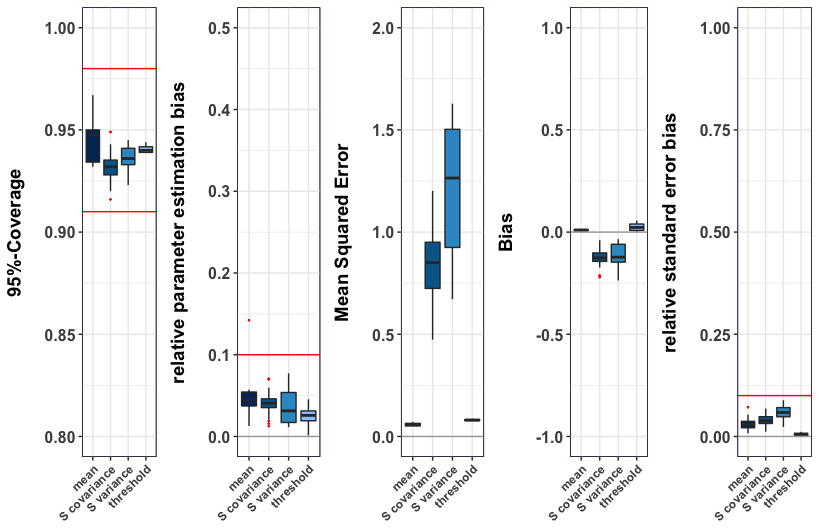
\includegraphics[width=1\textwidth]{Boxplot_LatentState_freeSvar_5categ.png}
   \end{center}
    \end{adjustwidth}
      \captionsetup{skip=10pt,width=1.05\textwidth}
\caption[Results LS 5 categ]{Results of the simulation study for the Latent State (LS) model including one construct with freely estimated latent State variances and covariances, spanning 9 measurement time points. Ordinal indicators were simulated with 5 ordered categories. Boxplots display the distribution of the respective statistic across different parameters of the same parameter type.}
\label{Fig: LS one free 5 categ}
\end{figure}

  \subsubsection{Freely varying state variances and covariances across time points. 7 ordered categories.}
  
 \begin{figure}[H]
 \begin{adjustwidth}{-1cm}{-1cm}
    \begin{center}
  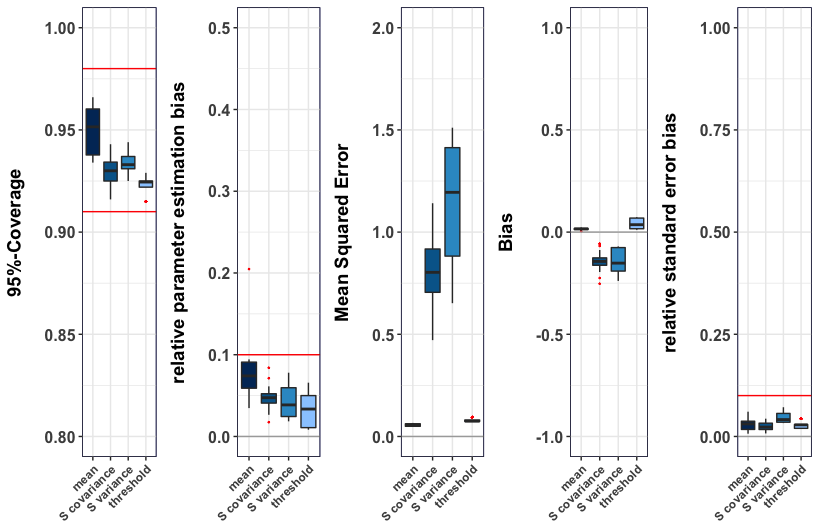
\includegraphics[width=1\textwidth]{Boxplot_LatentState_freeSvar_7categ.png}
   \end{center}
    \end{adjustwidth}
      \captionsetup{skip=10pt,width=1.05\textwidth}
\caption[Results LS 7 categ]{Results of the simulation study for the Latent State (LS) model including one construct with freely estimated latent State variances and covariances, spanning 9 measurement time points. Ordinal indicators were simulated with 7 ordered categories. Boxplots display the distribution of the respective statistic across different parameters of the same parameter type.}
\label{Fig: LS one free 7 categ}
\end{figure}


\subsection{Latent State Trait models: One construct}
  \subsubsection{Fixed state variances across time points. Default priors.}

 \begin{figure}[H]
 \begin{adjustwidth}{-1cm}{-1cm}
    \begin{center}
  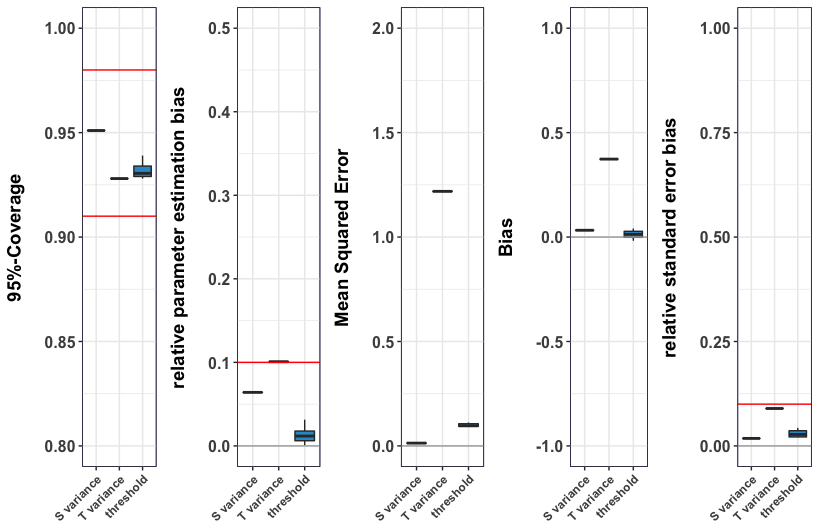
\includegraphics[width=1\textwidth]{Boxplot_LST_fixed.png}
   \end{center}
    \end{adjustwidth}
      \captionsetup{skip=10pt,width=1.05\textwidth}
\caption[Results LST fixed variance]{Results of the simulation study for the Latent State Trait (LST) model including one construct with latent state residual variances fixed to be equal across time, spanning 9 measurement time points. MPlus default priors. Ordinal indicators were simulated with 7 ordered categories. Boxplots display the distribution of the respective statistic across different parameters of the same parameter type.}
\label{Fig: LST one fixed}
\end{figure}


  \subsubsection{Fixed state variances across time points. Inverse gamma priors.}

 \begin{figure}[H]
 \begin{adjustwidth}{-1cm}{-1cm}
    \begin{center}
  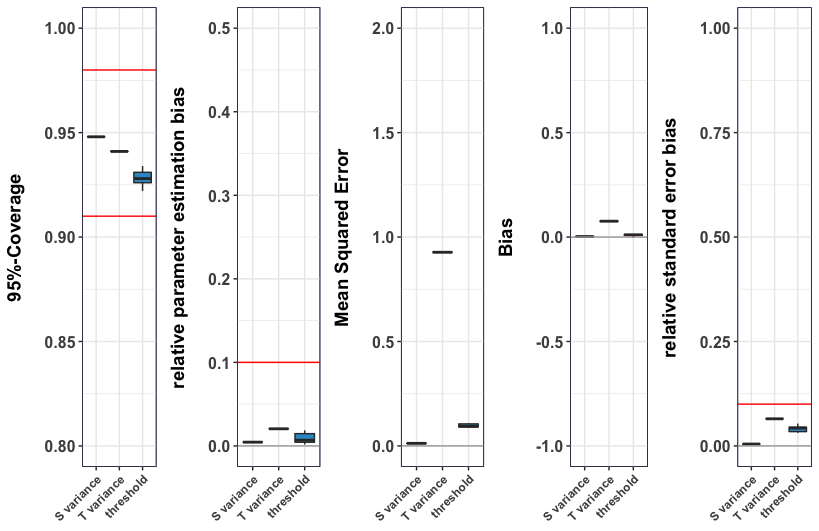
\includegraphics[width=1\textwidth]{Boxplot_LST_fixed_IGprior.png}
   \end{center}
    \end{adjustwidth}
      \captionsetup{skip=10pt,width=1.05\textwidth}
\caption[Results LST fixed variance IG]{Results of the simulation study for the Latent State Trait (LST) model including one construct with latent state residual variances fixed to be equal across time, spanning 9 measurement time points. Inverse gamma priors IG(0.001,0.001) for all variances. Ordinal indicators were simulated with 7 ordered categories. Boxplots display the distribution of the respective statistic across different parameters of the same parameter type.}
\label{Fig: LST one fixed IG}
\end{figure}


  \subsubsection{Free state variances across time points. Default priors.}


 \begin{figure}[H]
 \begin{adjustwidth}{-1cm}{-1cm}
    \begin{center}
  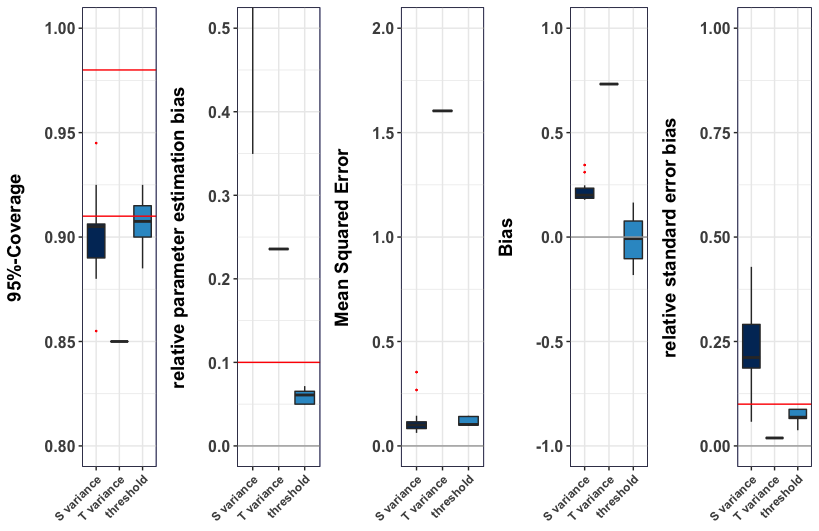
\includegraphics[width=1\textwidth]{Boxplot_LST_free.png}
   \end{center}
    \end{adjustwidth}
      \captionsetup{skip=10pt,width=1.05\textwidth}
\caption[Results LST free variance]{Results of the simulation study for the Latent State Trait (LST) model including one construct with latent state residual variances freely estimates across time, spanning 9 measurement time points.  Ordinal indicators were simulated with 7 ordered categories. Boxplots display the distribution of the respective statistic across different parameters of the same parameter type.}
\label{Fig: LST one free}
\end{figure}

  \subsubsection{Free state variances across time points. Inverse gamma priors.}

 \begin{figure}[H]
 \begin{adjustwidth}{-1cm}{-1cm}
    \begin{center}
  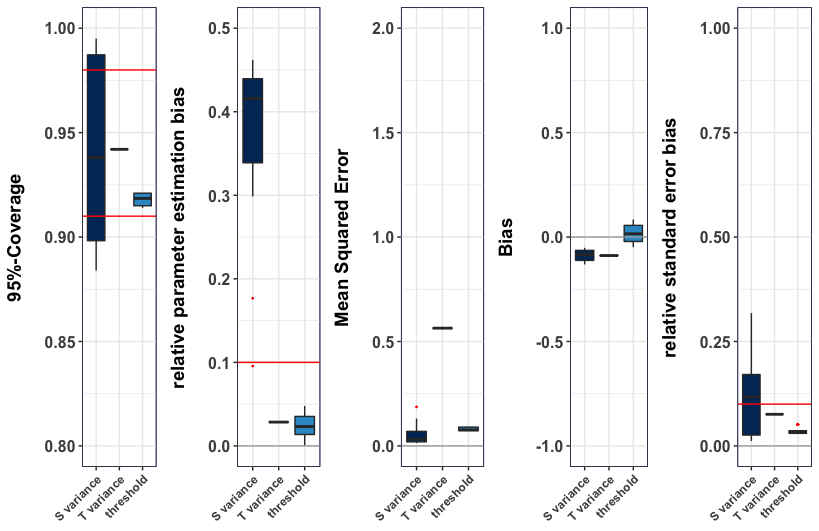
\includegraphics[width=1\textwidth]{Boxplot_LST_free_IGprior.png}
   \end{center}
    \end{adjustwidth}
      \captionsetup{skip=10pt,width=1.05\textwidth}
\caption[Results LST free variance IG]{Results of the simulation study for the Latent State Trait (LST) model including one construct with latent state residual variances freely estimates across time, spanning 9 measurement time points. Inverse gamma priors IG(0.001,0.001) for all variances. Ordinal indicators were simulated with 7 ordered categories. Boxplots display the distribution of the respective statistic across different parameters of the same parameter type.}
\label{Fig: LST one free IG}
\end{figure}

\subsection{Latent State models: Two constructs}
 \subsubsection{Free state variances and covariances across time points. Default priors.}

 \begin{figure}[H]
 \begin{adjustwidth}{-1cm}{-1cm}
    \begin{center}
  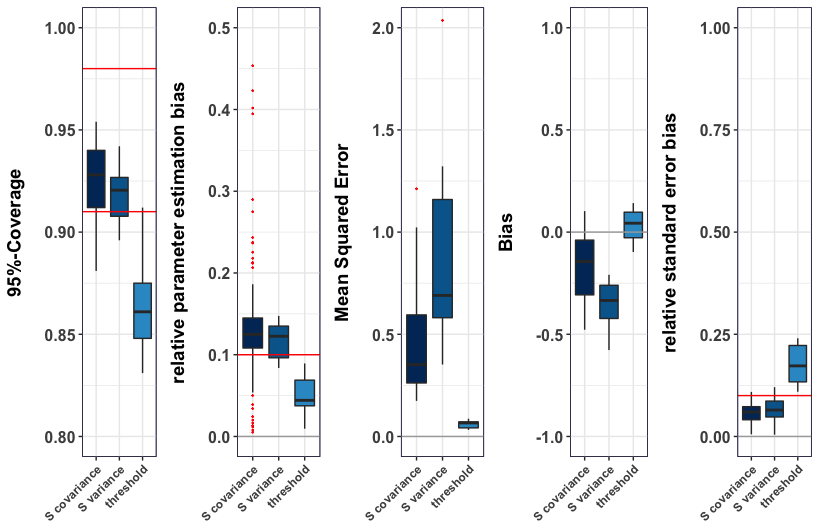
\includegraphics[width=1\textwidth]{Boxplot_Latent_State_2construcs_free.png}
   \end{center}
    \end{adjustwidth}
      \captionsetup{skip=10pt,width=1.05\textwidth}
\caption[Results LS free variance two constructs]{Results of the simulation study for the Latent State model including two constructs with latent state variances freely estimates across time, spanning 9 measurement time points.  Ordinal indicators were simulated with 7 ordered categories. Boxplots display the distribution of the respective statistic across different parameters of the same parameter type.}
\label{Fig: LS free}
\end{figure}

\subsection{Latent State Trait models: Two constructs}

 \subsubsection{Free state variances and covariances across time points.}
 
  \begin{figure}[H]
 \begin{adjustwidth}{-1cm}{-1cm}
    \begin{center}
  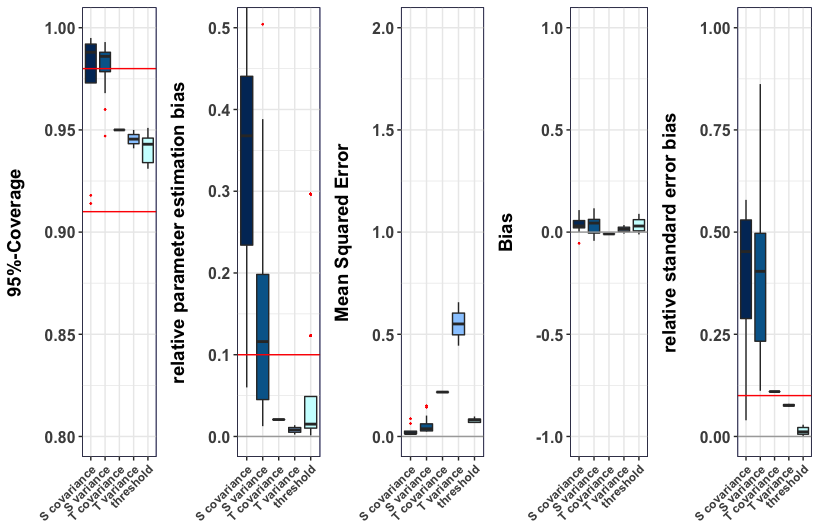
\includegraphics[width=1\textwidth]{Boxplot_LST_2constructs_freeSvar.png}
   \end{center}
    \end{adjustwidth}
      \captionsetup{skip=10pt,width=1.05\textwidth}
\caption[Results LST free variance two constructs]{Results of the simulation study for the Latent State Trait (LST) model including two constructs with free latent state residual variances across time, spanning 9 measurement time points.  Ordinal indicators were simulated with 7 ordered categories. Boxplots display the distribution of the respective statistic across different parameters of the same parameter type.}
\label{Fig: LST two free}
\end{figure}


 \subsubsection{Fixed state variances and covariances across time points.}

 \begin{figure}[H]
 \begin{adjustwidth}{-1cm}{-1cm}
    \begin{center}
  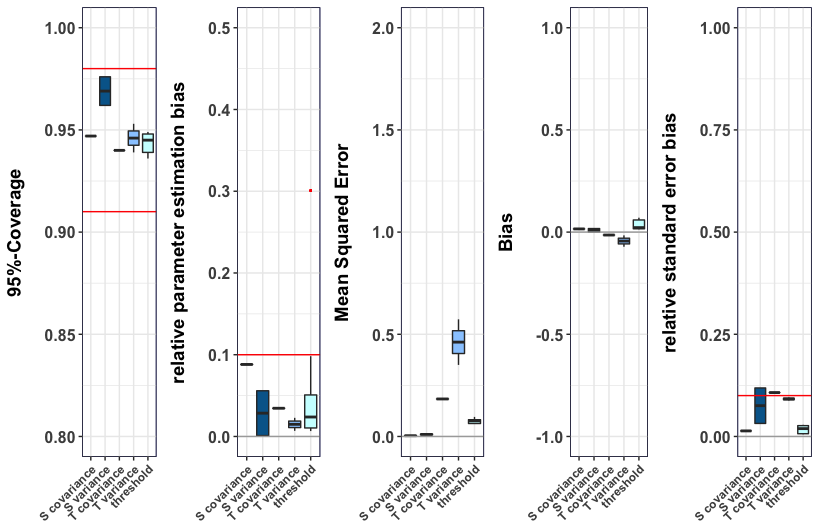
\includegraphics[width=1\textwidth]{Boxplot_LST_2constructs_fixed.png}
   \end{center}
    \end{adjustwidth}
      \captionsetup{skip=10pt,width=1.05\textwidth}
\caption[Results LST fixed variance two constructs]{Results of the simulation study for the Latent State Trait (LST) model including two constructs with fixed latent state residual variances across time, spanning 9 measurement time points.  Ordinal indicators were simulated with 7 ordered categories. Boxplots display the distribution of the respective statistic across different parameters of the same parameter type.}
\label{Fig: LST two fixed}
\end{figure}






% literature
\bibliography{literature}

\end{document}
